% document class and packages
\documentclass{beamer}
%\usepackage{adjustbox}
%\usepackage{algorithm,algorithmic}
%\usepackage{amsmath}
%\usepackage{amssymb}
%\usepackage{graphicx}
%\usepackage{hyperref}
\usepackage{listings}
\usepackage{textcomp}
\usepackage{color}
\usepackage{pgfplots}
\pgfplotsset{compat=newest}
\usepgfplotslibrary{fillbetween}
\usetikzlibrary{arrows,decorations.markings}

% indent for algorithm pseudo-code
\newlength\myindent
\setlength\myindent{1em}
\newcommand\bindent{%
  \begingroup
  \setlength{\itemindent}{\myindent}
  \addtolength{\algorithmicindent}{\myindent}
}
\newcommand\eindent{\endgroup}

% remove figure caption prefix
\setbeamertemplate{caption}{\raggedright\insertcaption\par}

% hyperlinks setup
\hypersetup{colorlinks,breaklinks,
	urlcolor=[rgb]{0,0.75,1},
	linkcolor=[rgb]{0.75,0.75,0.75}}

% empty navigation symbols
\beamertemplatenavigationsymbolsempty

% remove navigation dots on miniframes
\makeatletter
\def\beamer@writeslidentry{\clearpage\beamer@notesactions}
\makeatother

% Use Theme
\usetheme{Warsaw}
\useoutertheme[footline=authortitle]{miniframes}
\useinnertheme[shadow=true]{rounded}

% Colors
\definecolor{black}{RGB}{0,0,0} % black
\definecolor{dgreen}{RGB}{0,73,73} % dark green
\definecolor{lgreen}{RGB}{0,146,146} % light green
\definecolor{dpink}{RGB}{255,109,182} % dark pink
\definecolor{lpink}{RGB}{255,182,119} % light pink
\definecolor{dpurple}{RGB}{73,0,146} % dark purple
\definecolor{dblue}{RGB}{0,109,219} % dark blue
\definecolor{lpurple}{RGB}{182,109,255} % light purple
\definecolor{lblue}{RGB}{109,182,255} % light blue
\definecolor{pblue}{RGB}{182,219,255} % powder blue
\definecolor{dred}{RGB}{146,0,0} % dark red
\definecolor{brown}{RGB}{146,73,0} % brown
\definecolor{orange}{RGB}{219,209,0} % orange
\definecolor{bgreen}{RGB}{36,255,36} % bright green
\definecolor{yellow}{RGB}{255,255,109} % yellow

% Beamer Colors
\setbeamercolor{palette primary}{bg=black,fg=black!10}
\setbeamercolor{palette secondary}{bg=lblue,fg=black!10}
\setbeamercolor{palette tertiary}{bg=black,fg=black!10}
\setbeamercolor{structure}{fg=black}
\setbeamercolor{frametitle}{fg=black}

\lstset{upquote=true}
\lstdefinestyle{python}
{
	backgroundcolor=\color{dblue},	% choose the background color; you must add \usepackage{color} or \usepackage{xcolor}; should come as last argument
	basicstyle=\scriptsize,        	% the size of the fonts that are used for the code
	breakatwhitespace=false,        	% sets if automatic breaks should only happen at whitespace
	breaklines=true,                 	% sets automatic line breaking
	captionpos=b,                    	% sets the caption-position to bottom
  	commentstyle=\color{pblue},    	% comment style
	deletekeywords={...},            	% if you want to delete keywords from the given language
	escapeinside={\%*}{*)},          	% if you want to add LaTeX within your code
	extendedchars=true,              	% lets you use non-ASCII characters; for 8-bits encodings only, does not work with UTF-8
	firstnumber=1000,                	% start line enumeration with line 1000
	frame=single,	                   	% adds a frame around the code
	keepspaces=true,                 	% keeps spaces in text, useful for keeping indentation of code (possibly needs columns=flexible)
	keywordstyle=\color{orange},   	% keyword style
	language=Python,                 	% the language of the code
	morekeywords={...},			% if you want to add more keywords to the set
	numbers=none,                    	% where to put the line-numbers; possible values are (none, left, right)
	numbersep=5pt,                   	% how far the line-numbers are from the code
	numberstyle=\tiny\color{dpink},	% the style that is used for the line-numbers
	rulecolor=\color{black},         	% if not set, the frame-color may be changed on line-breaks within not-black text (e.g. comments (green here))
	showspaces=false,                	% show spaces everywhere adding particular underscores; it overrides 'showstringspaces'
	showstringspaces=false,        	% underline spaces within strings only
	showtabs=false,                  	% show tabs within strings adding particular underscores
	stepnumber=2,                    	% the step between two line-numbers. If it's 1, each line will be numbered
	stringstyle=\color{bgreen},		% string literal style
	tabsize=2,	                   		% sets default tabsize to 2 spaces
	title=\lstname                   		% show the filename of files included with \lstinputlisting; also try caption instead of title
}

% Title Page
\title{Hillside and Spectral Rankability}
\author{Thomas R. Cameron}
\institute{Davidson College}
\date{June 25, 2019}

\begin{document}
% Title Frame
\begin{frame}
	\titlepage
\end{frame}

%%%%%%%%%%%%%%%%%%%%%%%%%%%%%%%%%%%%%%%%%%%%%%%%%%%%%%
%								Big East CFB
%%%%%%%%%%%%%%%%%%%%%%%%%%%%%%%%%%%%%%%%%%%%%%%%%%%%%%
\section{Big East CFB}

\begin{frame}{Spectral Rankability}
\centering
\resizebox{0.80\textwidth}{!}{% Big East CFB
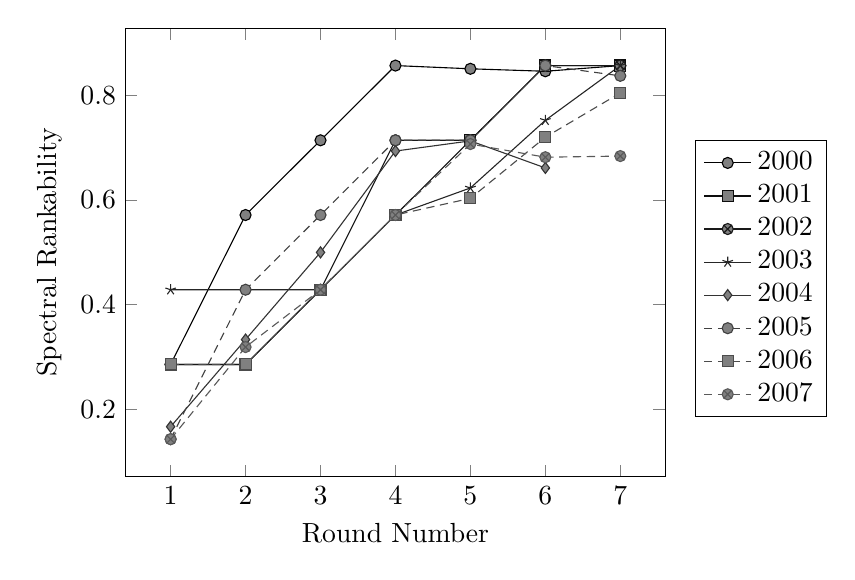
\begin{tikzpicture}
	\begin{axis}[
		xlabel = Round Number,
		ylabel =  Spectral Rankability,
		legend style={at={(1.3,0.75)}},
		cycle list name = black white]
		\addplot+[black] coordinates{
			(1,0.285714286)
			(2,0.571428571)
			(3,0.714285714)
			(4,0.857142857)
			(5,0.850996283)
			(6,0.846274058)
			(7,0.857142857)
		};
		\addplot+[black!95] coordinates{
			(1,0.285714286)
			(2,0.285714286)
			(3,0.428571429)
			(4,0.571428571)
			(5,0.714285714)
			(6,0.857142857)
			(7,0.857142857)
		};
		\addplot+[black!90] coordinates{
			(1,0.285714286)
			(2,0.285714286)
			(3,0.428571429)
			(4,0.714285714)
			(5,0.714285714)
			(6,0.857142857)
			(7,0.857142857)
		};
		\addplot+[black!85] coordinates{
			(1,0.428571429)
			(2,0.428571429)
			(3,0.428571429)
			(4,0.571428571)
			(5,0.623177997)
			(6,0.752509829)
			(7,0.857142857)
		};
		\addplot+[black!80] coordinates{
			(1,0.166666667)
			(2,0.333333333)
			(3,0.5)
			(4,0.693726496)
			(5,0.713173191)
			(6,0.661459403)
		};
		\addplot+[black!75] coordinates{
			(1,0.142857143)
			(2,0.428571429)
			(3,0.571428571)
			(4,0.714285714)
			(5,0.714285714)
			(6,0.857142857)
			(7,0.83751713)
		};
		\addplot+[black!70] coordinates{
			(1,0.285714286)
			(2,0.285714286)
			(3,0.428571429)
			(4,0.571428571)
			(5,0.603319894)
			(6,0.720219423)
			(7,0.804853514)
		};
		\addplot+[black!65] coordinates{
			(1,0.142857143)
			(2,0.318969374)
			(3,0.428571429)
			(4,0.571428571)
			(5,0.707099952)
			(6,0.68194562)
			(7,0.684131683)
		};
		\legend{2000,2001,2002,2003,2004,2005,2006,2007}
	\end{axis}
\end{tikzpicture}%
}
\end{frame}

\begin{frame}{Hillside Rankability}
\centering
\resizebox{0.80\textwidth}{!}{% Big East CFB
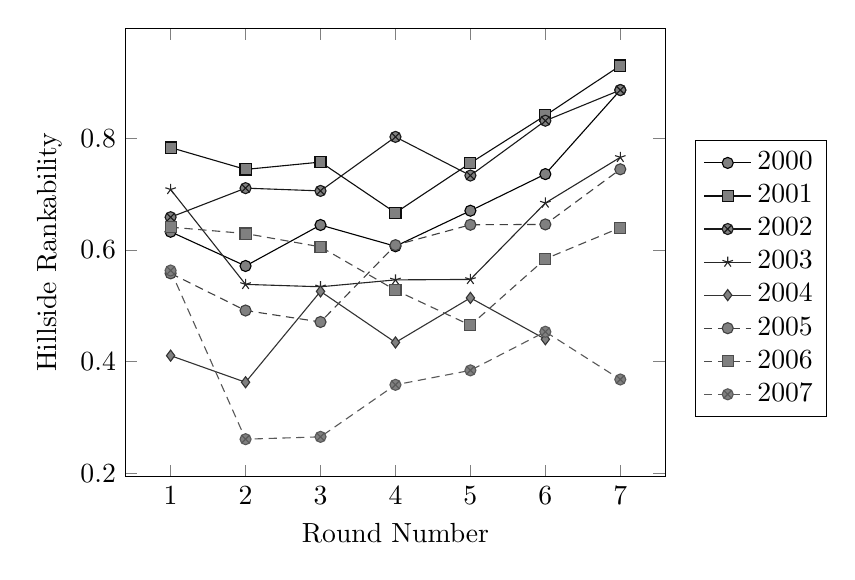
\begin{tikzpicture}
	\begin{axis}[
		xlabel = Round Number,
		ylabel =  Hillside Rankability,
		legend style={at={(1.3,0.75)}},
		cycle list name = black white]
		\addplot+[black] coordinates{
			(1,0.632590298)
			(2,0.571343537)
			(3,0.644704861)
			(4,0.606651284)
			(5,0.670263169)
			(6,0.735825484)
			(7,0.886275703)
		};
		\addplot+[black!95] coordinates{
			(1,0.783317246)
			(2,0.744211018)
			(3,0.757350289)
			(4,0.666633598)
			(5,0.75566399)
			(6,0.840867379)
			(7,0.930094131)
		};
		\addplot+[black!90] coordinates{
			(1,0.658698593)
			(2,0.710691392)
			(3,0.705777311)
			(4,0.802449233)
			(5,0.733260582)
			(6,0.831378188)
			(7,0.886275703)
		};
		\addplot+[black!85] coordinates{
			(1,0.708298198)
			(2,0.53840812)
			(3,0.534140574)
			(4,0.546484519)
			(5,0.547286967)
			(6,0.684108709)
			(7,0.765881459)
		};
		\addplot+[black!80] coordinates{
			(1,0.410837438)
			(2,0.363203463)
			(3,0.525898079)
			(4,0.434437543)
			(5,0.514297386)
			(6,0.44021164)
		};
		\addplot+[black!75] coordinates{
			(1,0.558158263)
			(2,0.491656909)
			(3,0.471124111)
			(4,0.608665459)
			(5,0.645145289)
			(6,0.645769263)
			(7,0.74445922)
		};
		\addplot+[black!70] coordinates{
			(1,0.64083486)
			(2,0.62944224)
			(3,0.60557372)
			(4,0.528037498)
			(5,0.465208039)
			(6,0.584100464)
			(7,0.639873016)
		};
		\addplot+[black!65] coordinates{
			(1,0.563265306)
			(2,0.261304945)
			(3,0.265506329)
			(4,0.358624482)
			(5,0.384500916)
			(6,0.453658693)
			(7,0.368201754)
		};
		\legend{2000,2001,2002,2003,2004,2005,2006,2007}
	\end{axis}
\end{tikzpicture}%
}
\end{frame}

\begin{frame}{Correlation Matrix}
\[
\textrm{corrcoef([eloCorr,specR,hillR])} = 
\begin{bmatrix}
1 & 0.911 & 0.899 \\
0.911 & 1 & 0.894 \\
0.899 & 0.894 & 1
\end{bmatrix}
\]
\end{frame}


\end{document}